\documentclass[12pt,letterpaper]{article}

\usepackage[utf8]{inputenc}
\usepackage[T1]{fontenc}
\usepackage{amsmath}
\usepackage{amsfonts}
\usepackage{amssymb}
\usepackage{amsthm}
\usepackage[left=2cm,right=2cm,top=2cm,bottom=2cm,headheight=22pt]{geometry}
\usepackage{fancyhdr}
\usepackage{setspace}
\usepackage{lastpage}
\usepackage{graphicx}
\usepackage{caption}
\usepackage{subcaption}
\usepackage{paralist}
\usepackage{url}

\theoremstyle{definition}
\newtheorem{question}{Question}
\newtheorem{example}{Example}
\newtheorem{exercise}[question]{Exercise}
\newtheorem*{challenge}{Challenge}
\newtheorem*{theorem}{Theorem}
\newtheorem*{definition}{Definition}

\begin{document}

%Paramètres de mise en forme des paragraphes selon les normes françaises
\setlength{\parskip}{1ex plus 0.5ex minus 0.2ex}
\setlength{\parindent}{0pt}

%Paramètres relatifs aux en-têtes et pieds de page.
\pagestyle{fancy}
\lhead{Theron J Hitchman}
\chead{\Large Reading and Guided Practice \#08}
\rhead{Spring 2016}
\lfoot{\emph{Math and Decision Making }}
\cfoot{}
\rfoot{\emph{\thepage\ of \pageref{LastPage}}}

\section*{Introduction}

Here you will learn a bit more about graph coloring problems. And you will revisit the idea of \emph{isomorphism}
for graphs.

\section*{Goals}
At the end of this assignment, a student should be able to:
\begin{compactitem}
\item Use graph colorings to tell graphs apart.
\item State an interesting theorem about the chromatic number of a planar graph.
\item Check when two (smallish) graphs are isomorphic by making a correspondence between vertices.
\end{compactitem}
A student might also be able to:
\begin{compactitem}
\item Solve a challenging set of tasks about graph colorings and isomorphisms.
\end{compactitem}

\section*{Reading and Questions for Graphs Day 09}

It has been important to us all unit to think about the fact that a graph represents some network, where all that matters is ``how things are connected.'' What does generally matter is \textit{how the graph is drawn}. If we rearrange things without changing the internal connections, we think of it as the same graph. We ran across this
notion pretty early in our study, and we called graphs \emph{isomorphic} when they are essentially the same thing.

Recall that two graphs, $G$ and $H$ are called \emph{isomorphic} when there is a way to make the
vertices of $G$ correspond to the vertices of $H$ in a one-to-one way, so that for each pair of vertices $v$ and $w$
in $G$ and their corresponding vertices $x$ and $y$ in $H$,  $v$ and $w$ are joined by an edge exactly when $x$ and $y$ are joined by an edge.

\begin{exercise}\label{ex:iso}
Make an example of a pair of isomorphic graphs that have drawings that look different. Check the definition above. 
How does your correspondence work?
\end{exercise}

\begin{exercise}
Make an example of a pair of graphs, each with four vertices, which are NOT isomorphic.
\end{exercise}

\subsection*{Graph colorings as invariants}

One of the ways we can use graph colorings, or better, chromatic numbers of graphs, is as an invariant.
What does that mean? Well, if two
graphs are isomorphic, which means one is just a redrawing of the other, then a $k$-coloring of one graph 
should correspond to a $k$-coloring of the other graph. (Just pull the colors through the correspondence between
vertices! Try it with your example from Exercise \ref{ex:iso}.) 

\begin{exercise}
Work out why this means that the chromatic number of a graph is an invariant, too.
\end{exercise}

So we can use the existence or non-existence of a certain type of coloring as a way to say for sure that a pair of
graphs are \textbf{not} isomorphic. For example here are two graphs, each with 5 vertices and 8 edges.

\begin{figure}[h]
\centering
\begin{subfigure}[b]{0.4\textwidth}
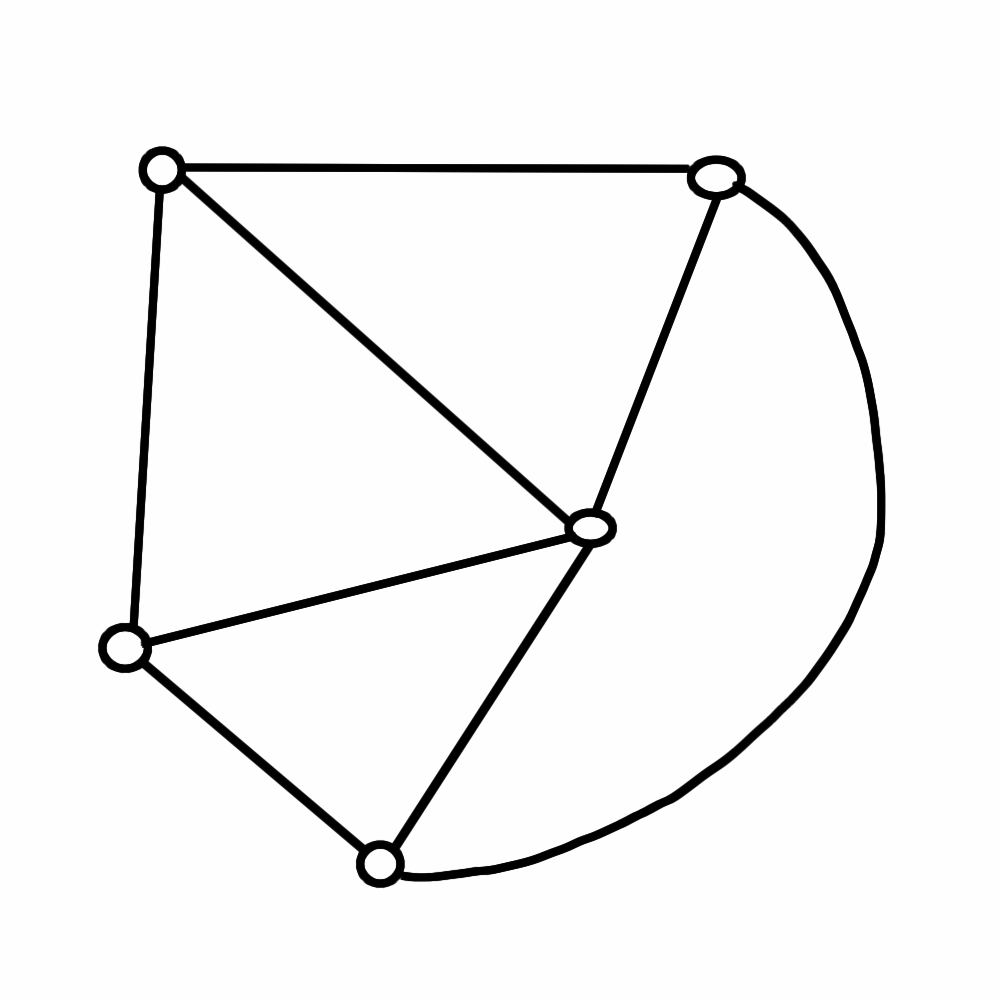
\includegraphics[width=\textwidth]{images/tricolor.png}
\caption{Graph A with 5 vertices and 8 edges}
\label{fig:3color}
\end{subfigure}
\qquad
\begin{subfigure}[b]{0.4\textwidth}
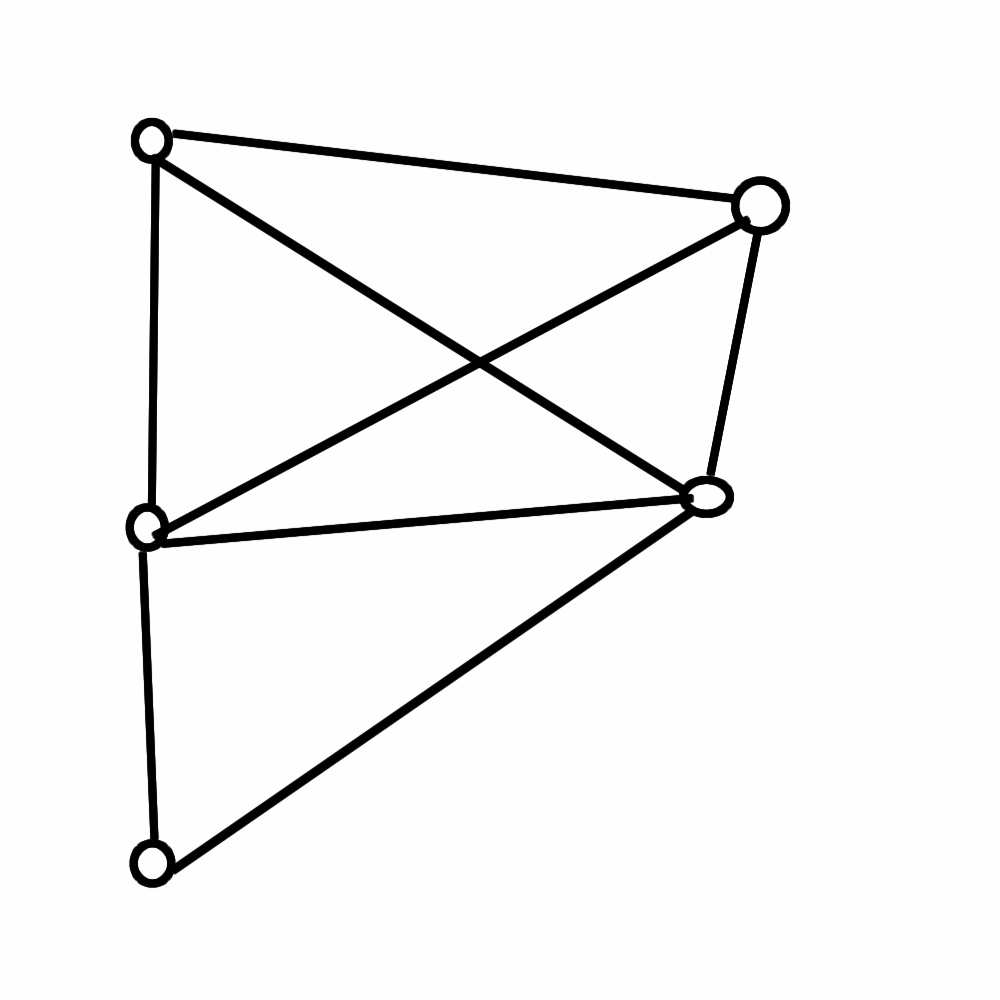
\includegraphics[width=\textwidth]{images/4color.png}
\caption{Graph B with 5 vertices and 8 edges}
\label{fig:4color}
\end{subfigure}
\caption{Non-isomorphic Graphs}
\label{fig:noniso}
\end{figure}

How can we be so sure that these graphs are non-isomorphic? Well, Graph A has a 3-coloring. But Graph B does not have a 3-coloring. Therefore, these two graphs must be truly different.

\begin{exercise}
Find a 3-coloring for Graph A.
\end{exercise}

\begin{exercise}
Find a subgraph of Graph B which is a copy of $K_4$, the complete graph on 4 vertices. Use this to explain why 
Graph B cannot have a 3-coloring.
\end{exercise}

Now, if you were paying attention, there is another way we know how to tell these graphs apart. 

\begin{exercise}
Find the degree sequences of Graph A and Graph B. Use this information to say why the graphs are not isomorphic.
\end{exercise}

\begin{challenge}
Find an example of a pair of graphs which have (1) the same number of vertices, (2) the same number of edges, 
(3) the same degree sequences, but (4) have different chromatic numbers. 

This pair of graphs is not isomorphic.
\end{challenge}

\begin{challenge}[Super Challenge] 
Find an example of a pair of graphs which have (1) the same number of vertices, (2) the same number of edges, 
(3) the same degree sequences, and (4) the same chromatic number, but (5) are still not isomorphic.
\end{challenge}


\clearpage
\subsection*{An Important Theorem}

Mathematicians have made a pretty thorough study of the chromatic numbers of graphs, and discovered some amazing things. One of these facts has an interesting history. Let's start with the statement.

\begin{theorem}[The Four Color Theorem] 
The chromatic number of a planar graph is no bigger than 4. That is, if $G$ is a planar graph, then $G$ has a
4-coloring.
\end{theorem}

The (known) history of this theorem goes like this: This property was noticed in the 1850s by man (named Guthrie)
who was making a map of the counties of England. He started asking around about it. People took it as a conjecture, 
rather than as a question. In 1879 a man named Kempe published an argument and claimed the theorem. In 1880
another, independent, argument was given by a man named Tait.  By 1891, both proofs had been thrown out
because readers had (eventually) found flaws. In particular, a man named Heawood found the flaw in Kempe's proof, 
and then proved that 5 colors would suffice (and a bunch of other stuff). Things stood like this until 1976, when
Kenneth Appel and Wolfgang Haken built upon some ideas of Heinrich Heesch to write a \emph{computer-based}
proof!

This was a controversial thing. Appel and Haken found a way to reduce the problem to a situation where they had 
to check a large number of cases (almost 2000 of them). They programmed a computer to do the checking for them.
This made mathematicians a bit uneasy. There are two purposes to writing a proof: (1) to convince people the
statement is true, and (2) explain in human terms why the statement is true. The computer proof definitely failed
on (2), and some people were not so sure about (1).  These days, we are feeling better about this particular theorem,
because it has been reworked by lots of other people since 1976. But still, the proof relies on using a computer.

\begin{challenge}
How does computer verification sound to you? Could you use a computer to convince yourself something is true?
What might you have to worry about? 
\end{challenge}

\begin{exercise}
Draw a map for a fantasy land of your choosing. You get to choose the countries and their boundaries. The only rule
is that each country has to be one connected piece.

Does your map have a 3-coloring? Since your drew a map on a sheet of paper, I am certain that it has a 4-coloring, 
even if it doesn't have a 3-coloring.

What do you have to do to make a map which \emph{requires} four colors?
\end{exercise}

\clearpage
\subsection*{More about Isomorphism of Graphs}

We have spent a lot of time figuring out how to say that graphs are not isomorphic. How do we say graphs are
isomorphic? We find a correspondence between the vertices which preserves edge connections. 
(Just like the definition says!)

\begin{exercise}
The graphs below are isomorphic. Find a way to label the vertices of the two graphs that shows how they correspond.
\begin{figure}[h]
\centering
\begin{subfigure}[b]{0.4\textwidth}
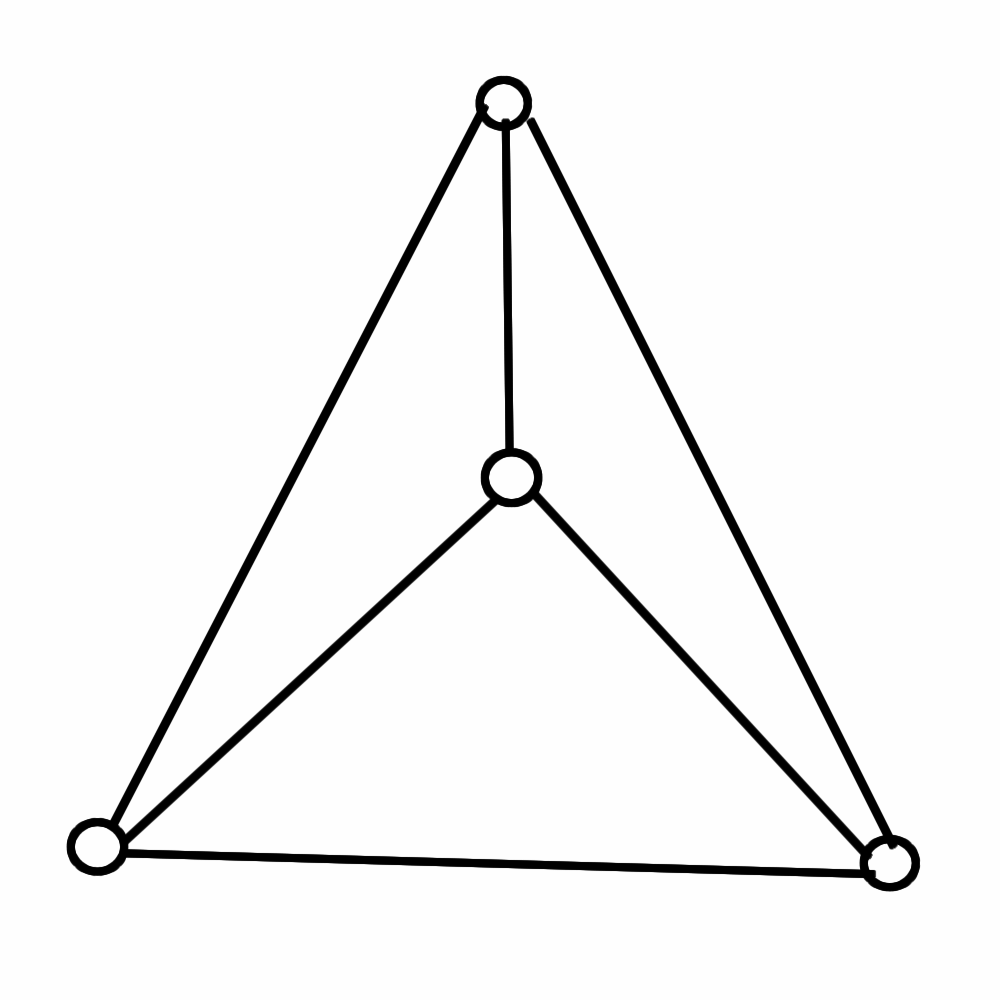
\includegraphics[width=\textwidth]{images/std_k4.png}
\caption{The graph $K_4$}
\end{subfigure}
\qquad
\begin{subfigure}[b]{0.4\textwidth}
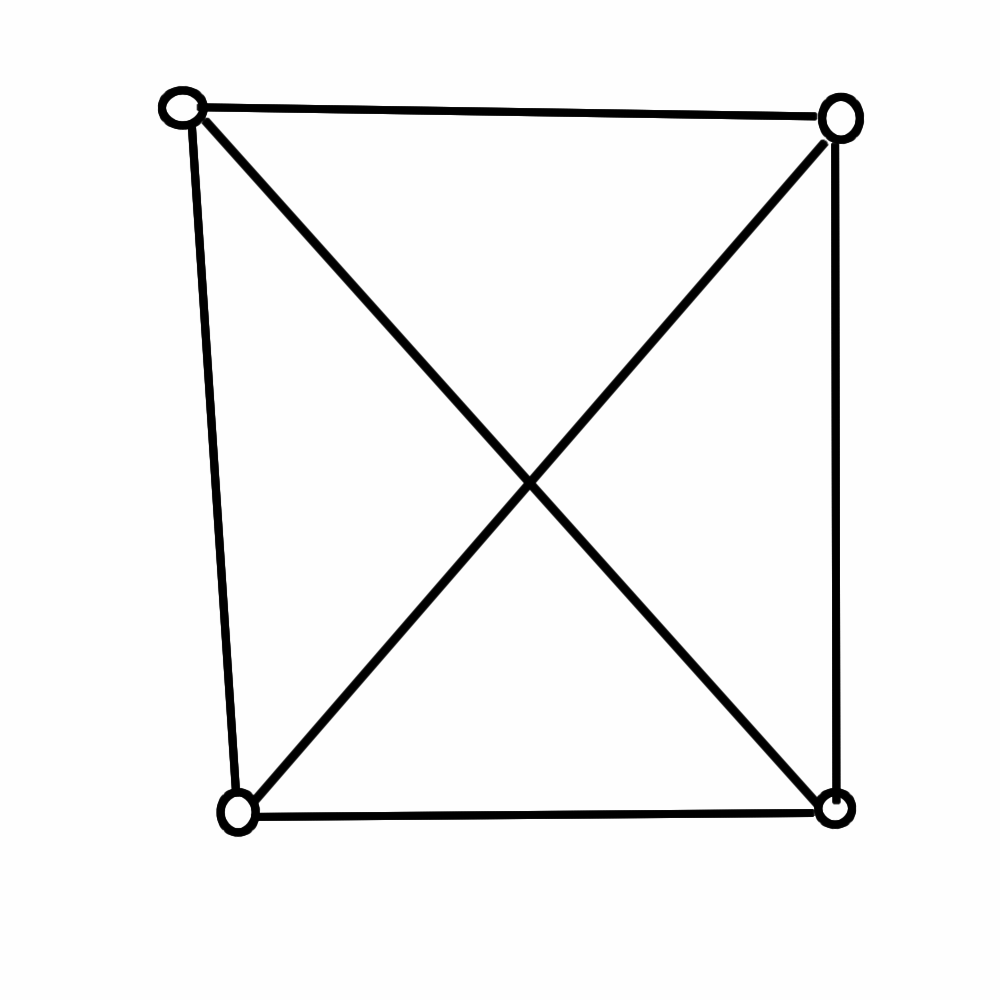
\includegraphics[width=\textwidth]{images/altk4.png}
\caption{Also $K_4$}
\end{subfigure}
\caption{Isomorphic Graphs}
\label{fig:k4}
\end{figure}
\end{exercise}

\begin{exercise}
The graphs below are isomorphic. Find a way to label the vertices of the two graphs that shows how they correspond.
\begin{figure}[h]
\centering
\begin{subfigure}[b]{0.4\textwidth}
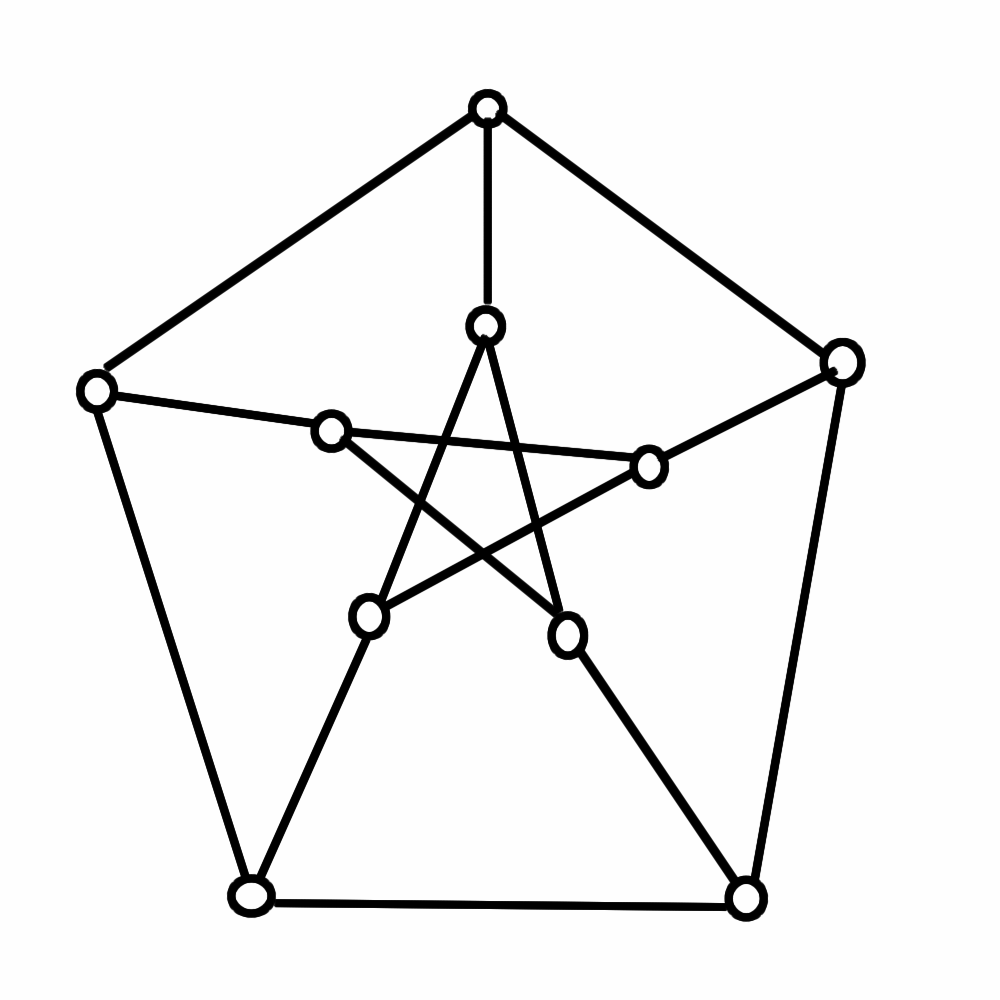
\includegraphics[width=\textwidth]{images/petersen-std.png}
\caption{The Petersen Graph}
\end{subfigure}
\qquad
\begin{subfigure}[b]{0.4\textwidth}
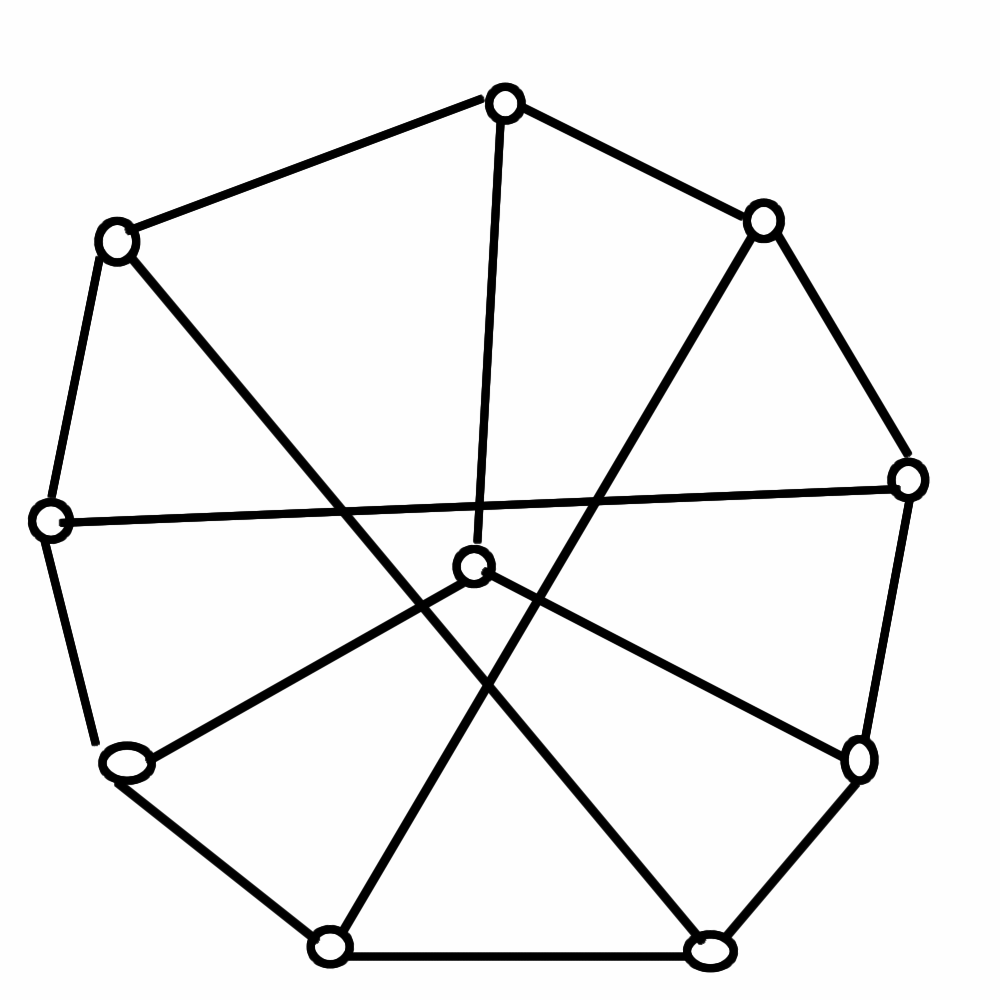
\includegraphics[width=\textwidth]{images/petersen-alt.png}
\caption{Also the Petersen Graph}
\end{subfigure}
\caption{Isomorphic Graphs}
\label{fig:petersen}
\end{figure}
\end{exercise}

\subsection*{A \emph{Really Recent} Announcement}


How could we program a computer to check that a pair of graphs is isomorphic?

\begin{challenge}
Think up a procedure for testing if two graphs are isomorphic. You don't have to write code,
but try to think of a process, an \emph{algorithm}, for checking this.
\end{challenge}


\noindent\textbf{Pause and try that for a bit. Really. Don't read on until you have given it some time.}

There is a straightforward way to go about it. First, ignore the edges and just make a list of all the possible ways to make the vertices of the two graphs to correspond. This list is likely to be very large. Then, for each of these possible
correspondences, go through all the different pairs of vertices and check if they agree on ``are these vertices connected or not.''

This na\"{i}ve approach will totally work. But it is slooooooooow. Really slow. If your graphs have a large number
of vertices, it will likely take too long to check. Your laptop will die before the computation is over.

So the problem becomes, ``Can we find a reasonably fast way to check if two graphs are isomorphic?''

In December of 2015, a major breakthrough was announced: Laslo Babai of the University of Chicago gave a series
of lectures in which he claimed
that he had found an algorithm for deciding if two graphs are isomorphic which works in \emph{quasipolynomial
time}. That is a technical way of saying ``pretty quickly, considering the size of the problem.''  It will likely be a while before the mathematics community decides to accept this as correct, but Babai has a pretty good reputation. 

Mathematics marches on. We learn more, and we get progress, even today.


%\begin{thebibliography}{9}
%\end{thebibliography}

\end{document}
%sagemathcloud={"zoom_width":100}